%!TEX root = main.tex
\section{System\label{sec:system}}
\subsection{Motivation and Objective}
While the concept of informativeness is useful for helping analysts determine which parent is the proper informative reference for a given visualization, in practice, users often do not have a preconceived knowledge of what visualizations would lead to useful insights. The ultimate goal of exploration is to discover insights, in particular finding visualizations that are \textit{interesting} and lead to those insights. %%during data exploration, % have a good idea of what visualizations they want to see. 
However, without knowing \textit{what} subset of data contains an insightful distribution, manually exploring distributions from all possible data subsets can be tedious and inefficient. In order to accelerate the process of manual drill-down, our goal is to develop a system that automatically selects a small set of \textit{interesting} visualizations to summarize the distributions within a dataset in an \textit{safe and informative} manner.
% accelerate the process of manual drill-down in a ``safe'' way by summarizing the 
% to discover the most informative and interesting stories within a dataset. We develop 
% an interactive visualization summarization system that automatically selects a small set of visualizations to summarize the distributions within a dataset in an informative manner.
% because analysts only have 
\par We first highlight three of the challenges (\textit{significance, safety, saliency}) that we face when building such a system and how they are each addressed in our system objective.
\stitle{Safety:} As discussed in Section~\ref{sec:datamodel}, failure to select the proper reference for a given visualization can lead to the drill-down fallacy. To resolve this issue, we require that for every visualization except for the overall, at least one of its informative parents must be included within the set of selected visualizations. This enforces that every selected reference visualization is guaranteed to be informative. %Additionally, we take preventive measures against the well-known problem of showing small subpopulations that could lead to spurious patterns and correlations~\cite{Binnig2017}. When constructing the visualization lattice, we allow users to select an `iceberg condition' \footnote{The terminology is used in the discussion of iceberg cubes in OLAP literature~\cite{Xin2007}.} ($\delta$) to adjust the extent of pruning on visualizations whose sizes fall below a certain percentage of the overall population size. Second, we downweigh the interestingness edge utility $D(V_i, V_i^j)$ between a parent $V_i^j$ and a child visualization $V_i$ by the ratio of their sizes  $U(V_i, V_i^j) = \frac{|V_i|}{|V_i^{j}|} \cdot D(V_i, V_i^j)$.
%Since showing multiple, improper parents can mislead users. %This enforces that every 
\stitle{Saliency:} We want to select visualizations that are \textit{visually-salient}, in other words, the visualization distribution is \textit{interesting} if differs from the distribution of its parents. The use of distance-based metrics to quantify surprisingness or interestingness have been widely adopted in past work~\cite{Vartak2015,Correll2016,Itti2009}. To model the interestingness of an visualization $V_i$ in the context of its parent $V_i^j$, we characterize the deviation between their data distributions using a distance function $D(V_i, V_i^j)$. From the safety criteria, all parents in the dashboard are guaranteed to be informative, therefore the reference would not be misleading. 
%visualization shown in the dashboard has an informative reference to compare against to create a connected story.
\stitle{Significance:} The danger of spurious patterns and correlations in visualizations that contain small subpopulation size is a well-known problem in exploratory analysis~\cite{Binnig2017}. We take two preventive measures to avoid picking these misleading visualizations that are `insignificant' in size. When constructing the visualization lattice, we allow users to select an `iceberg condition' \footnote{The terminology is used in the discussion of iceberg cubes in OLAP literature~\cite{Xin2007}.} ($\delta$) to adjust the extent of pruning on visualizations whose sizes fall below a certain percentage of the overall population size. Second, we downweigh the interestingness edge utility $D(V_i, V_i^j)$ between a parent $V_i^j$ and a child visualization $V_i$ by the ratio of their sizes  $U(V_i, V_i^j) = \frac{|V_i|}{|V_i^{j}|} \cdot D(V_i, V_i^j)$.

Given these objectives, we select $k$ visualization to include in our dashboard that represent a connected set of visualizations that are collectively safe, salient and significant, based on maximizing the utility $U(V_i, V_i^j)$. The problem of finding a connected subgraph in the lattice that has the maximum combined edge utility is known as the maximum-weight connected subgraph problem~\cite{ErnstAlthaus2009} and is known to be NP-Complete, via a reduction from the \textsc{Clique Problem}~\cite{Parameswaran2010}. Next, we discuss heuristic algorithms used for deriving a locally optimal solution for ensuring interactive runtime. 

% \textbf{Selective:} We select $k$ visualization to include in our dashboard that represent a connected set of visualizations that are collectively safe, salient and significant, based on maximizing the utility $U(V_i, V_i^j)$.
% \subsection{System Objective}
% Based on the concept of the informative parent developed in the last section, we wanted to develop an interactive dashboard that could help users understand key distributions in their dataset, while preventing the drill-down fallacy. We list several of the desired properties of the generated dashboard:
%  \begin{enumerate}
%   \item 
%   \item 
% % \begin{equation}
% %     U(V_i, V_i^j) = \frac{|V_i|}{|V_i^{j}|} \cdot D(V_i, V_i^j)
% %     \label{edge_utility}
% % \end{equation}

%   \item 
% \end{enumerate}
%Dashboard must include the overall visualization (topmost visualization with no filter applied) to serve as reference to the rest of the visualizations in the dashboard.
 
%\noindent Additional model extensions can be added to this objective function based user specification. For example, there may be $k$ visualizations that approximately yield equal contribution to the user's expectation. For simplicity of notation, we have assumed $k=1$ in the aforementioned model. In order, a user may want to prevent the recommendation of spuriously interesting subsets of the data. We can discard visualizations that falls below a certain subpopulation size threshold.
% \stitle{Subpopulation size consideration:} The danger of spurious patterns and correlations in visualizations that contain small subpopulation size is a well-known problem in exploratory analysis~\cite{Binnig2017}. We take two preventive measures to avoid including such misleading visualization in our dashboards. First, in the lattice generation process discussed in Section~\ref{sec:algorithms}, we allow users to select an `iceberg condition' \footnote{The terminology is used in the discussion of iceberg cubes in OLAP literature~\cite{Xin2007}.} ($\delta$) to adjust the extent of pruning on visualizations whose sizes fall below a certain percentage of the overall population size. Second, we downweigh the interestingness edge utility $U(V_i, V_i^j)$ between a parent $V_i^j$ and a child visualization $V_i$ by the ratio of their sizes:
% \begin{equation}
%     U(V_i, V_i^j) = \frac{|V_i|}{|V_i^{j}|} \cdot D(V_i, V_i^j)
%     \label{edge_utility}
% \end{equation}

% \subsection{System Architecture}
% We have implemented \system\ as a Flask web application on top of a PostgreSQL database. In Figure~\ref{system_architecture}, we present the system architecture of \system, which consists of three core modules: the traversal module, the query module, and the statistics module. The interaction manager deals with the supported user interaction described in Section~\ref{sec:interaction} and sends a request to the lattice module which  contains several algorithms for generating and traversing the visualization lattice described in Section~\ref{sec:algorithms}. For generating the visualization lattice, the lattice module passes a list of data subsets corresponding to visualizations to be generated to the query module. The query module translates these visualizations into queries, and then optimizes (by grouping) and executes the queries. The statistics module is an optional module that allows the lattice module to prune low-utility visualizations without actually generating them. Specifically, it generates coarse statistics for the unexplored visualizations based on the current list of explored visualizations. Finally, the dashboard renderer takes the resulting visualizations to be included in the dashboard and perform any rendering preprocessing procedures for display and navigation of the dashboard as described in Section \ref{sec:navigation}.
% \begin{figure}[ht!]
% \centering
% 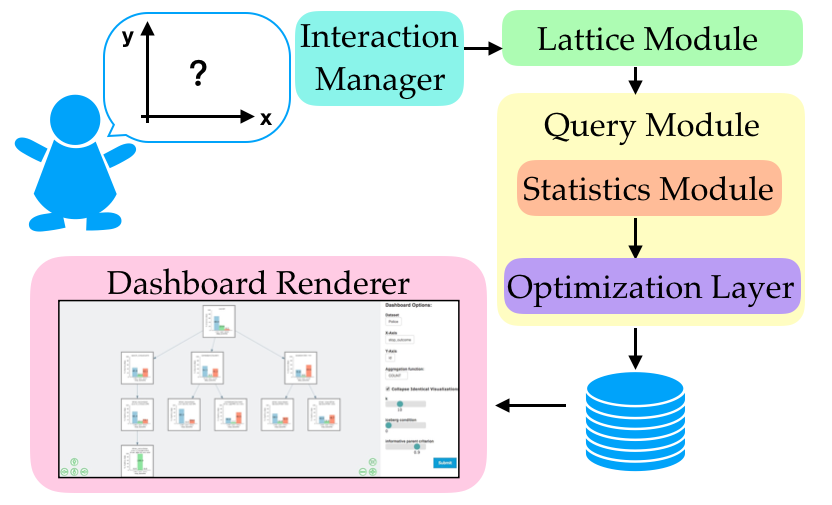
\includegraphics[width=\linewidth]{figures/system_architecture.png}
% \caption{System Architecture of \system. User starts with x and y axes of interest and requests for $k$ visualizations in the dashboard. The request is processed by generating the lattice with the help of the querying module, visualization selection through the lattice traversal algorithms, and finally the dashboard is displayed at the frontend through the dashboard renderer. }%  The interaction manager translates the request to the traversal module that ???? [should we look at the offline case??]}
% \label{system_architecture}
% \end{figure}

\subsection{Algorithms\label{sec:algorithms}}
We discuss algorithms used for generating the visualization lattice, and then present a high-level overview of our traversal algorithms to selecting the k-connected maximum-weighted subgraph.

\stitle{Lattice Generation:} Our system supports two variants of traversal algorithms based on the lattice generation procedure---offline variants that first generate the complete lattice and then work towards identifying the maximum utility solution, and online variants that incrementally generate the lattice and simultaneously identify the solution. The offline variants are appropriate for datasets with a small number of low-cardinality attributes, where we can generate the entire lattice in a reasonable time; whereas the online variants are appropriate for datasets with large number of high-cardinality attributes, where we incrementally generate a partial lattice.

%In most cases, the lattice contains a large number of visualizations due to the presence of many attributes or high-cardinality attributes in the dataset. In such cases finding an optimal solution is computationally challenging.

\stitle{Lattice Traversal:} Given the materialized lattice, the objective of the traversal algorithm is to find the connected subgraph in the lattice that has maximum combined edge utility. \cut{Here, we discuss the \textit{frontier greedy} algorithm which is used for generating the dashboards for our user study and defer the details of other algorithms that we have developed to the technical report.}
% \begin{figure}[ht!]
% \centering
% 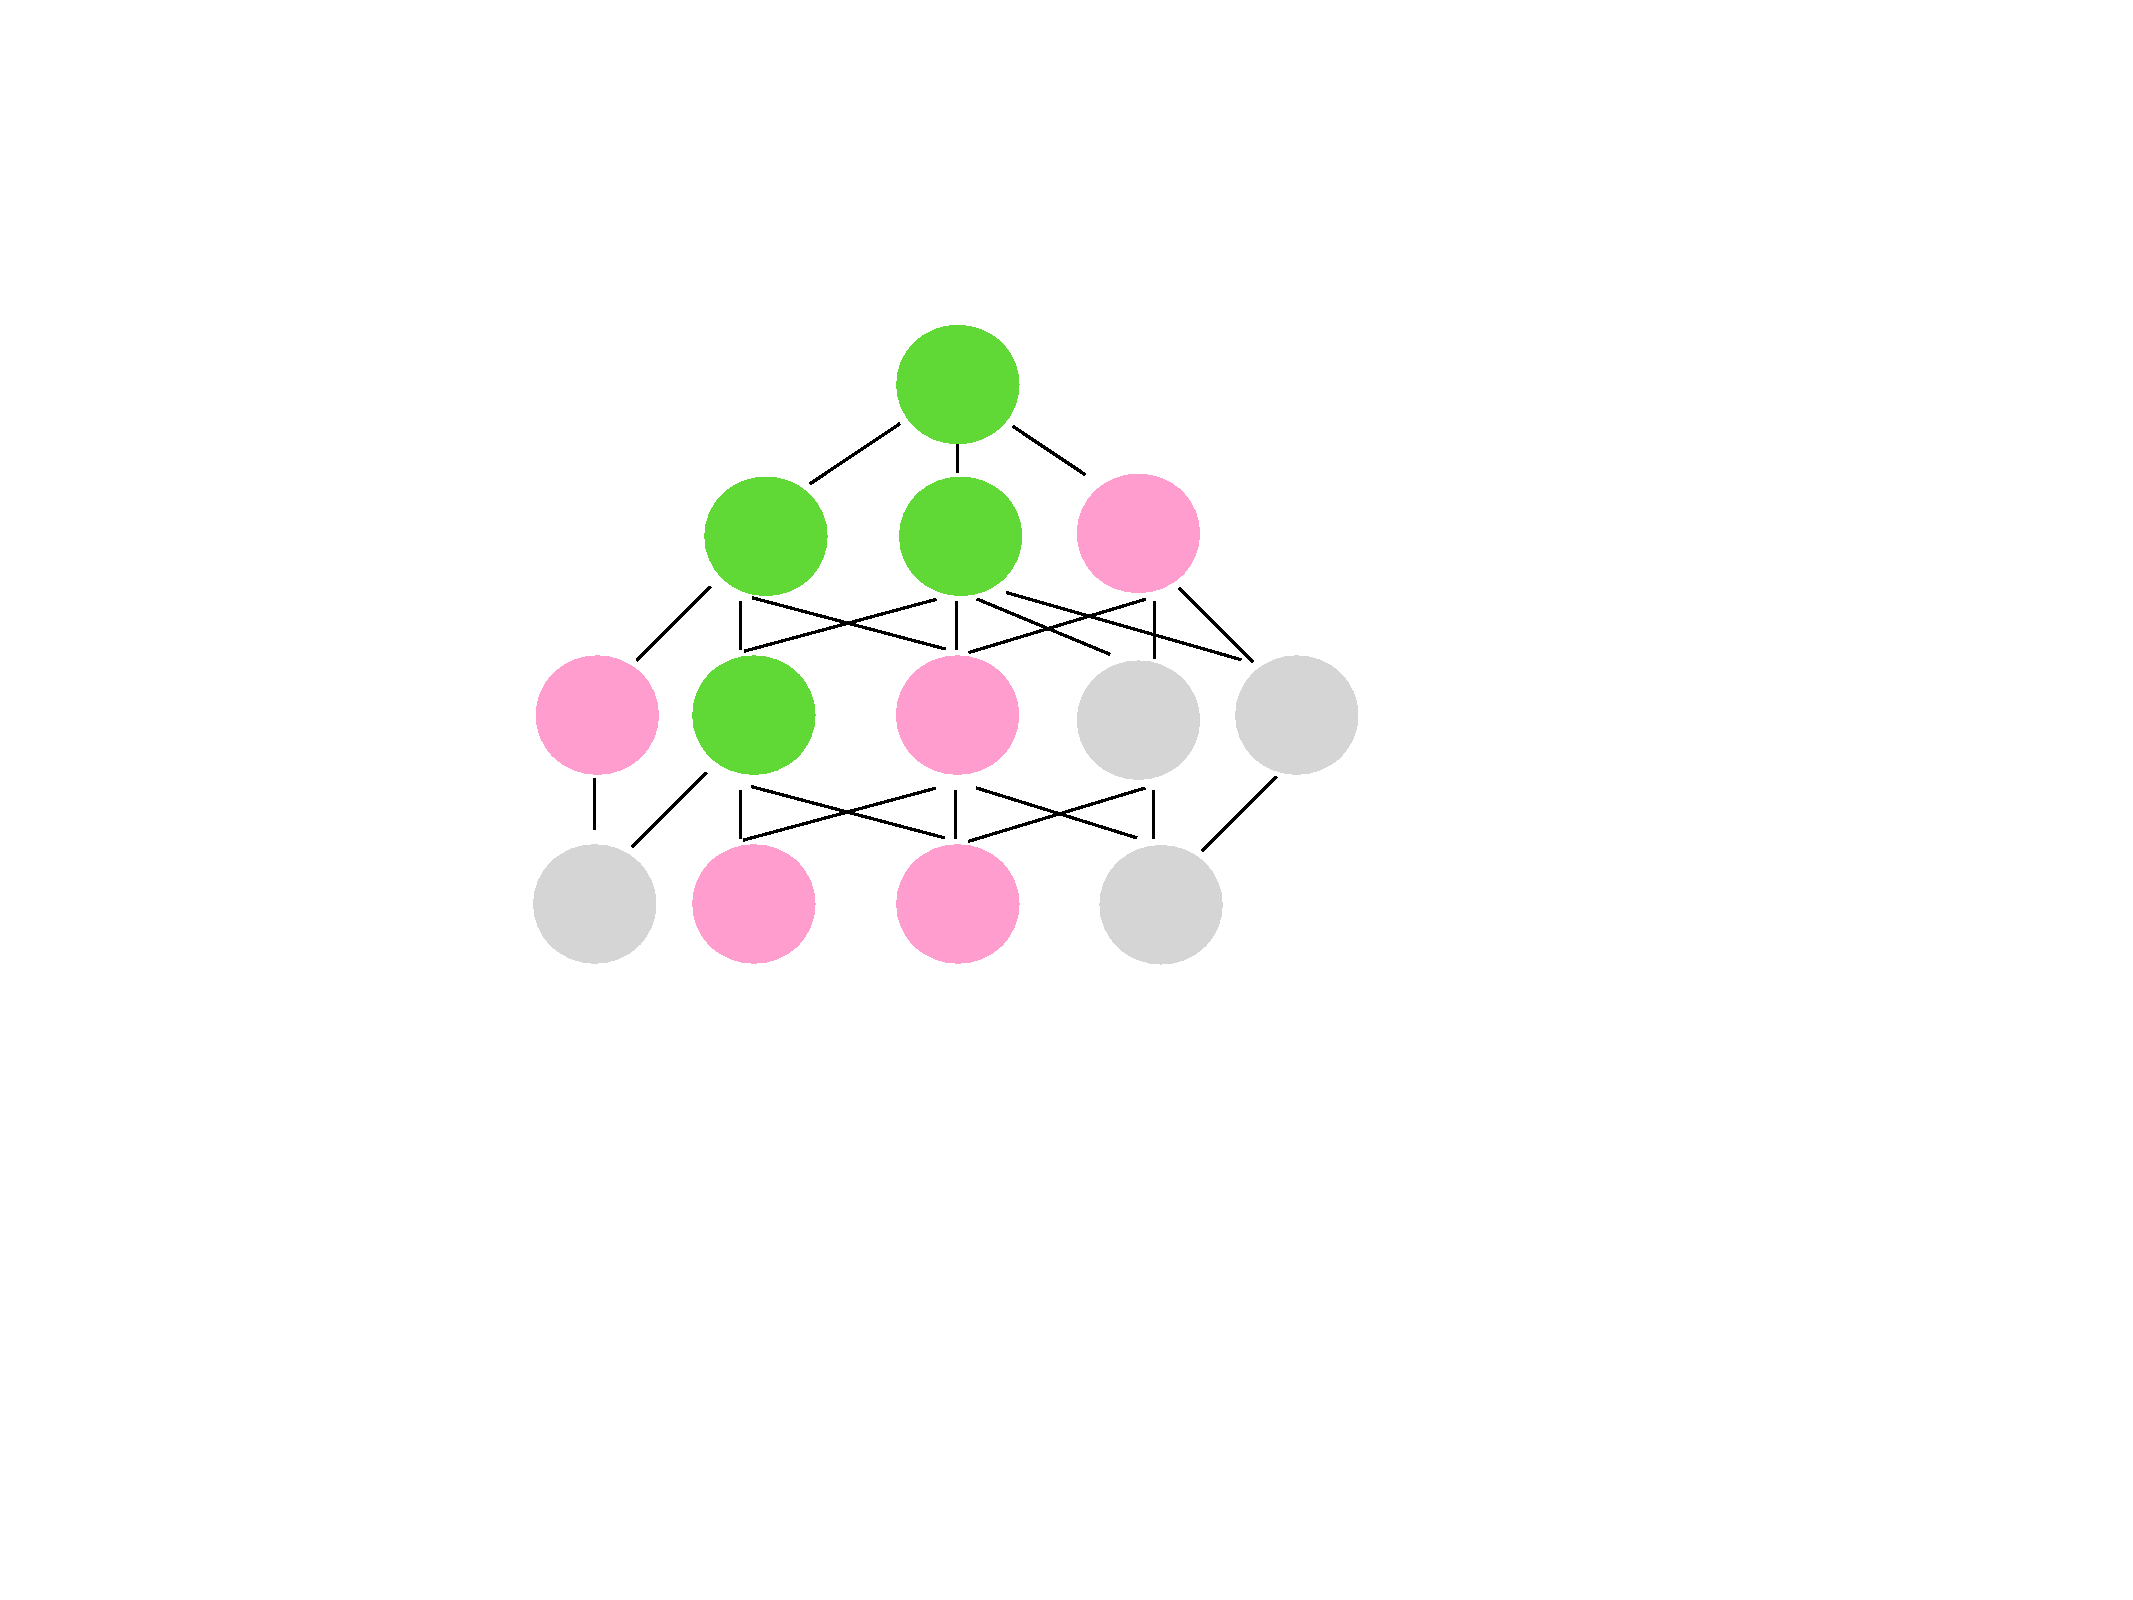
\includegraphics[width=0.4\linewidth]{figures/frontier.pdf}
% \caption{Toy example demonstrating the notion of ``frontier''. Nodes that have been picked to include in the dashboard are colored green. The neighbors of the set of picked nodes are the frontier nodes, shown in pink. Grey nodes are other unpicked nodes in the lattice.}
% \end{figure}
%We devised two classes of heuristics algorithms, namely, frontier-based algorithms, and path-merging algorithms. These algorithms are guaranteed to find a solution that satisfies the constraints of our problem, except for the optimality.
\techreport{The frontier-based algorithms traverse the lattice from root to downwards, incrementally adding new nodes (visualizations) to the current solution (dashboard) till it reaches the maximum capacity $k$. To achieve this, the algorithms maintain a list of candidate nodes---called \textit{frontier} nodes---any of which can be added to the current solution since their informative parent is already present in the solution. At each step, the algorithms add a node from frontier to the current solution, and update the frontier accordingly.  The frontier based algorithms can be further categorized into three types based on their node selection strategy (from frontier), namely greedy algorithm, random walk algorithm, and probabilistic algorithm. The greedy algorithm picks the current best node from frontier (thus concentrates on exploitation), random walk algorithm picks a random node (thus concentrates on exploration), and probabilistic algorithm picks a random high-utility node (thus trades off between exploration and exploitation).}
\par The frontier greedy algorithm obtains a list of candidate nodes known as the \textit{frontier} nodes, which encompasses all neighbors of nodes in the existing subgraph solution. Any of the nodes in the frontier can be added to the current solution since their informative parent is present in the solution. To obtain the frontier nodes, the algorithm scans and adds all children of leaf nodes of the current dashboard as part of the frontier. In the online version, it additionally checks for each child whether its informative parent is present in the current dashboard. At each step, our algorithm greedily picks the node with the maximum utility amongst the frontier nodes to add to the current solution, and updates the frontier accordingly.

\techreport{The path merging algorithm first generate the informative paths from root to every candidate node. Then, it greedily merges the paths with high-utility to create a subgraph whose size is less than or equal to maximum capacity $k$.}


\begin{algorithm}
  \begin{algorithmic}[1]
  \Procedure{pickVisualizations}{k,lattice}
  \State dashboard $\gets$ \{ $V_{overall}$ \}
  \While{|dashboard| < k}
      \State frontier $\gets$ getFrontier(dashboard,lattice)
      \State maxNode $\gets$ getMaxUtilityNode(frontier)
      \State dashboard $\gets$ dashboard $\cup$ \{maxNode\}
  \EndWhile
  \Return dashboard
  \EndProcedure
  \end{algorithmic}
  \caption{Frontier Greedy Algorithm}\label{algo:frontier_greedy}
\end{algorithm}

%\textbf{Greedy Algorithms:} Greedy algorithms select the locally optimal node to be added to the frontier.

%A specific implementation would need to specify a scoring function to nodes in frontier that is used to pop out the next node in each iteration. One can design a scoring function based on the trade-off between performance and complexity. In the most simple case, we can use the edge weights to score nodes in the frontier. That is, at each point we add a node with the highest interestingness value. We note that this is quite a greedy approach. Specifically, we might miss visualizations with high utility that are in deeper levels of the graph. Thus, another approach would be to extent the horizon for which we calculate a nodes utility. We denote such approach as a look-ahead approach. With a free parameter $n$, we would like to assign a score to each frontier node the corresponds to the expected utility of adding this node and $n-1$ more nodes who are its descendants. For example, we can run BFP for each node in frontier treating it as a root.

\subsection{User Interaction\label{sec:interaction}}
\begin{figure*}[ht!]
\centering
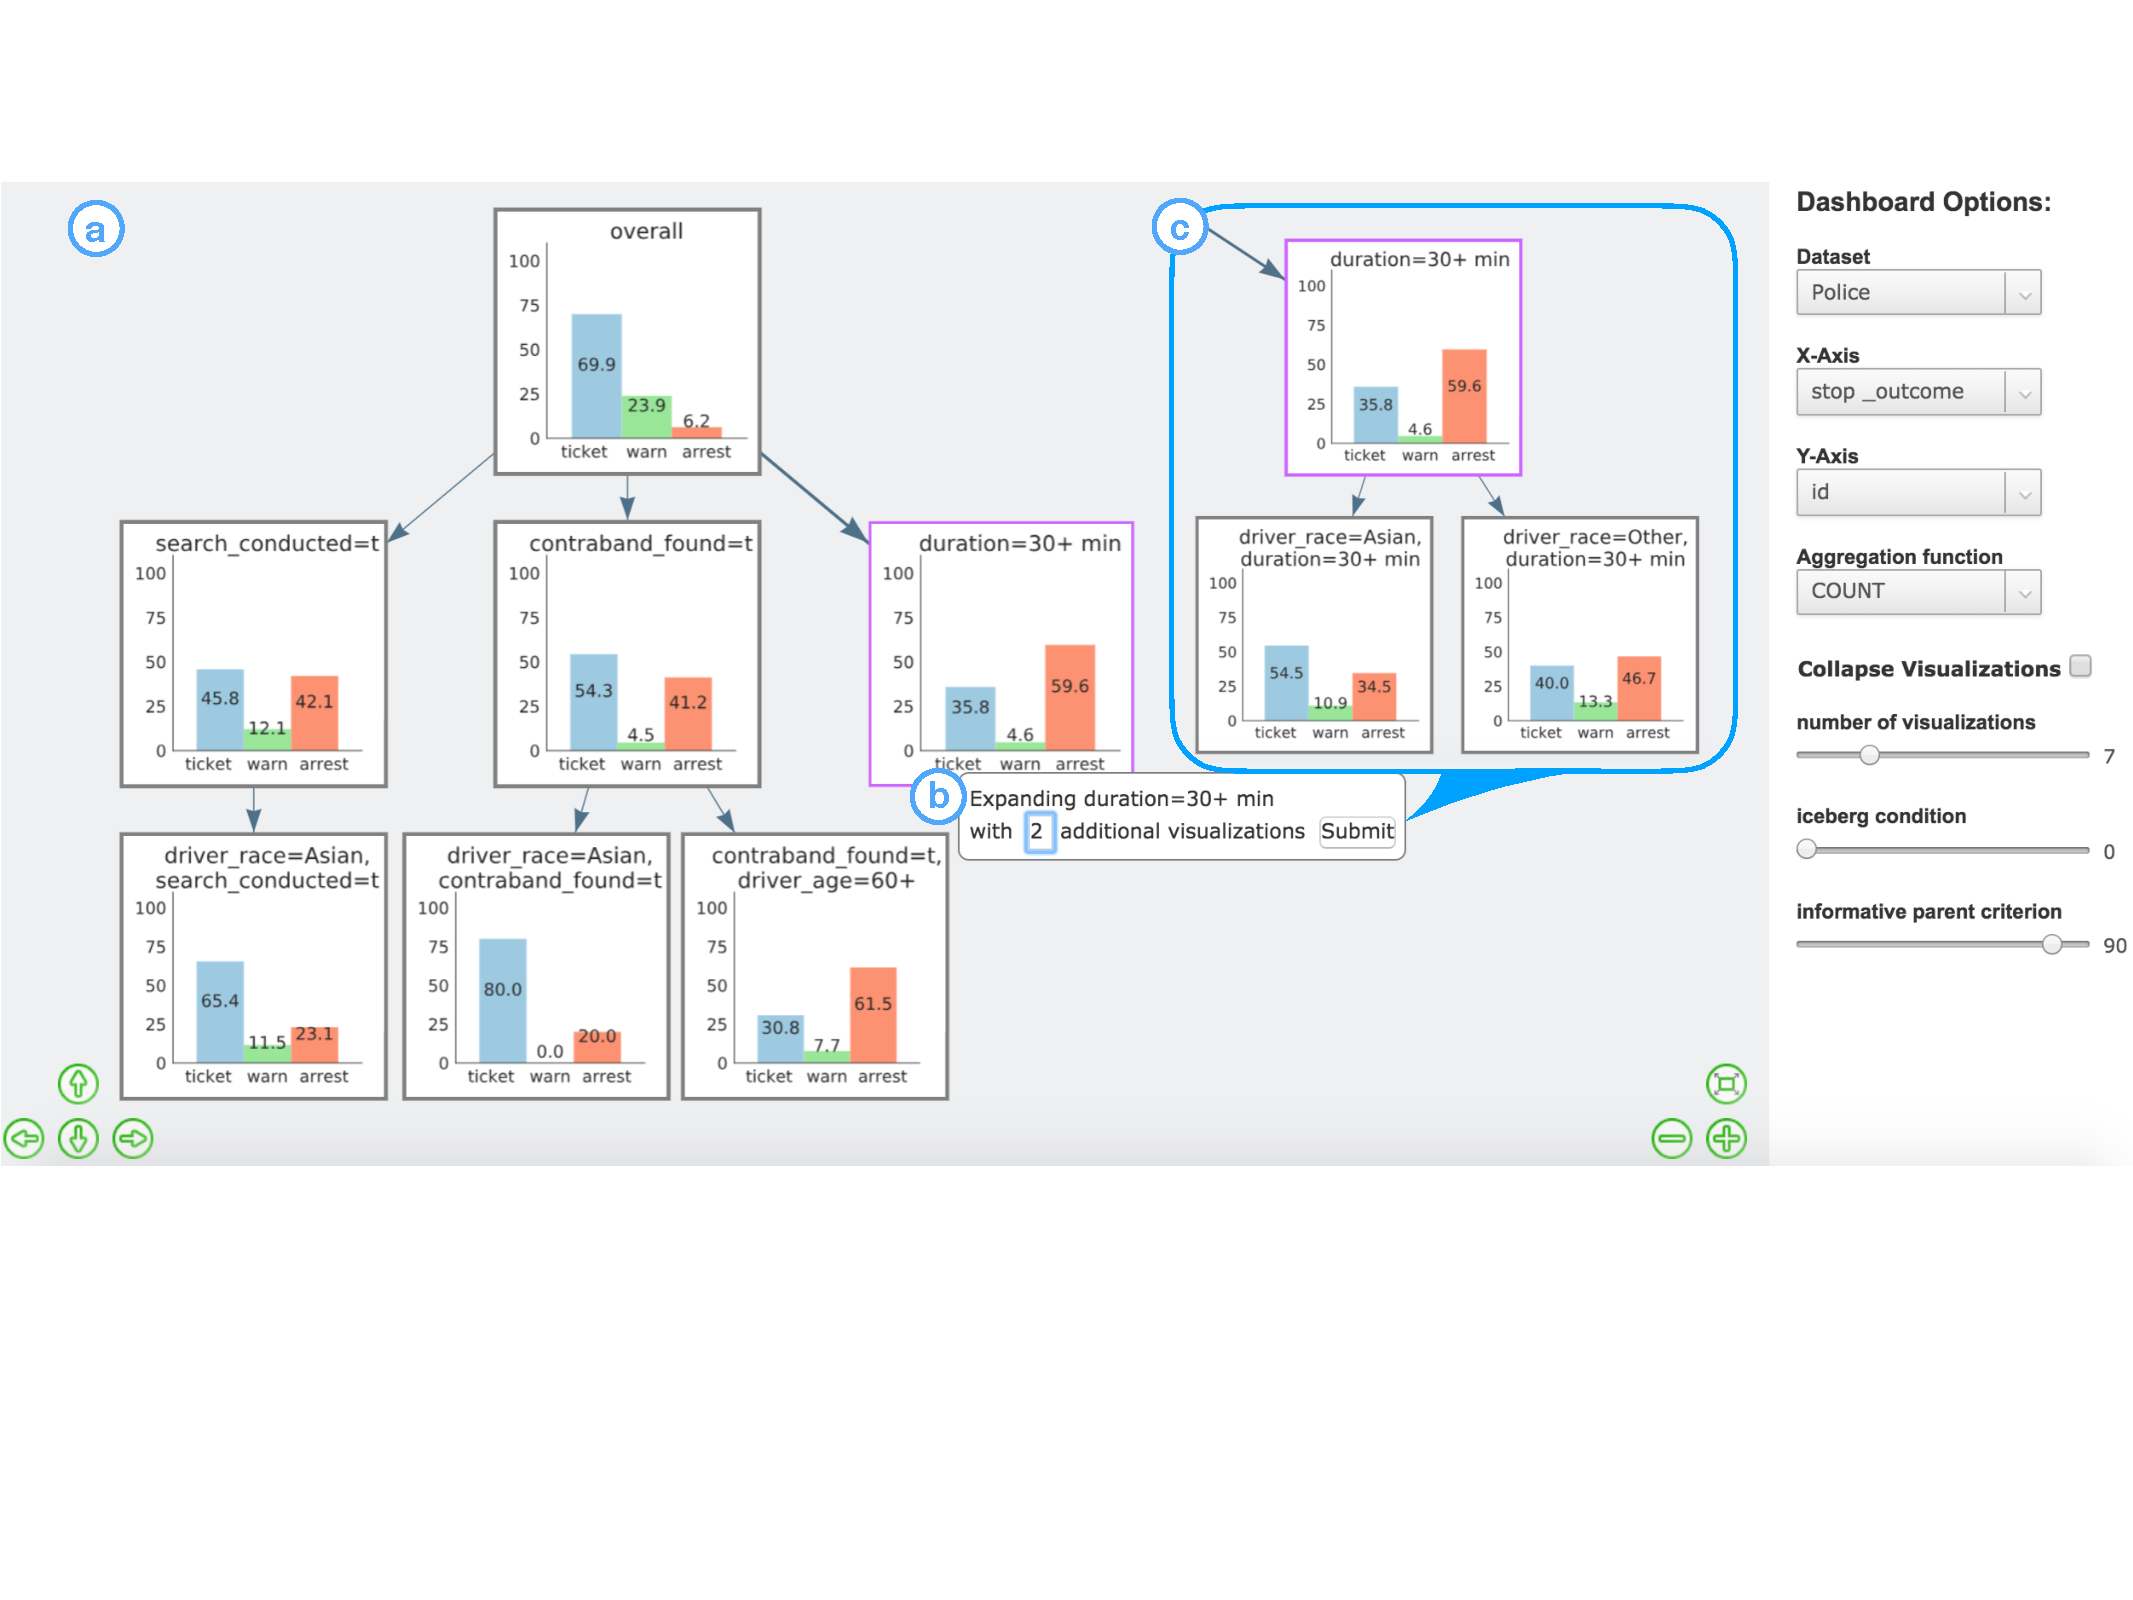
\includegraphics[width=0.8\linewidth,frame]{figures/overview_interface_expand.pdf}
\caption{a) Overview of the \system interface for the Police Stop dataset. Users can select x and y axes of interest, as well as a choice of an aggregation function. Default values are set for system related parameters such as the number of visualizations to show in the dashboard (k), iceberg condition for pruning ($\delta$), and informative parent criterion ($\theta$), which can be adjusted by the users via the sliders if needed. b) User clicks on the duration=30+min visualization to request 2 additional visualization. c) A preview of the added portion of the resulting dashboard is shown.}
\label{fig:overview}
\end{figure*}
\par Given the selected visualizations, we render the dashboard visualizations in an interactive frontend interface, as shown in Figure \ref{fig:overview}. The system allows users to inspect the visualization dashboard through panning and zooming with navigation buttons, mouse clicks, and keyboard bindings. Users can also select the x and y axes of interest, aggregation function, and optional system parameter settings to generate a dashboard.  
\par After browsing through visualizations in the dashboard, users may be interested in getting more information about a particular node. \system allows users to request additional summarizations based on a chosen visualization of interest as the new starting point for analysis. As shown in Figure \ref{fig:overview}a, the analyst starts with a 7-visualization dashboard on the Police Stop dataset~\cite{police}. The dataset contains records of vehicle and pedestrian stops from law enforcement departments in Connecticut, dated from 2013 to 2015. The analyst learns that for the drivers who had contraband found in the vehicle, the arrest rate for drivers who are 60 and over is surprisingly higher than usual, whereas for Asian drivers the arrest rate is lower. In addition, she is also interested in learning more about the other factor that contribute to high arrest rate: duration=30+min. In Figure~\ref{fig:overview}b, she clicks on the corresponding visualization and requests for 2 additional visualizations. Upon seeing the updated dashboard in Figure~\ref{fig:overview}c, she learns that similar to the selected visualization, any visualization that involves the duration=30+min filter results in high ticketing and arrest rates. This implies that if a police stop lasts more than 30 minutes, the outcome would more or less be the same, independent of factors such as driver's race or age. To generate the expanded dashboard, \system uses the same models and algorithms as before, except the root node is now set as the selected visualization, rather than the overall visualization. This node expansion capability is motivated by the idea of \textit{iterative view refinement} in other visual analytics system, which is essential for the users to iterate on and explore different hypotheses~\cite{Wongsuphasawat2016,Hoque2017}.

% \begin{figure}[ht!]
% \centering
% 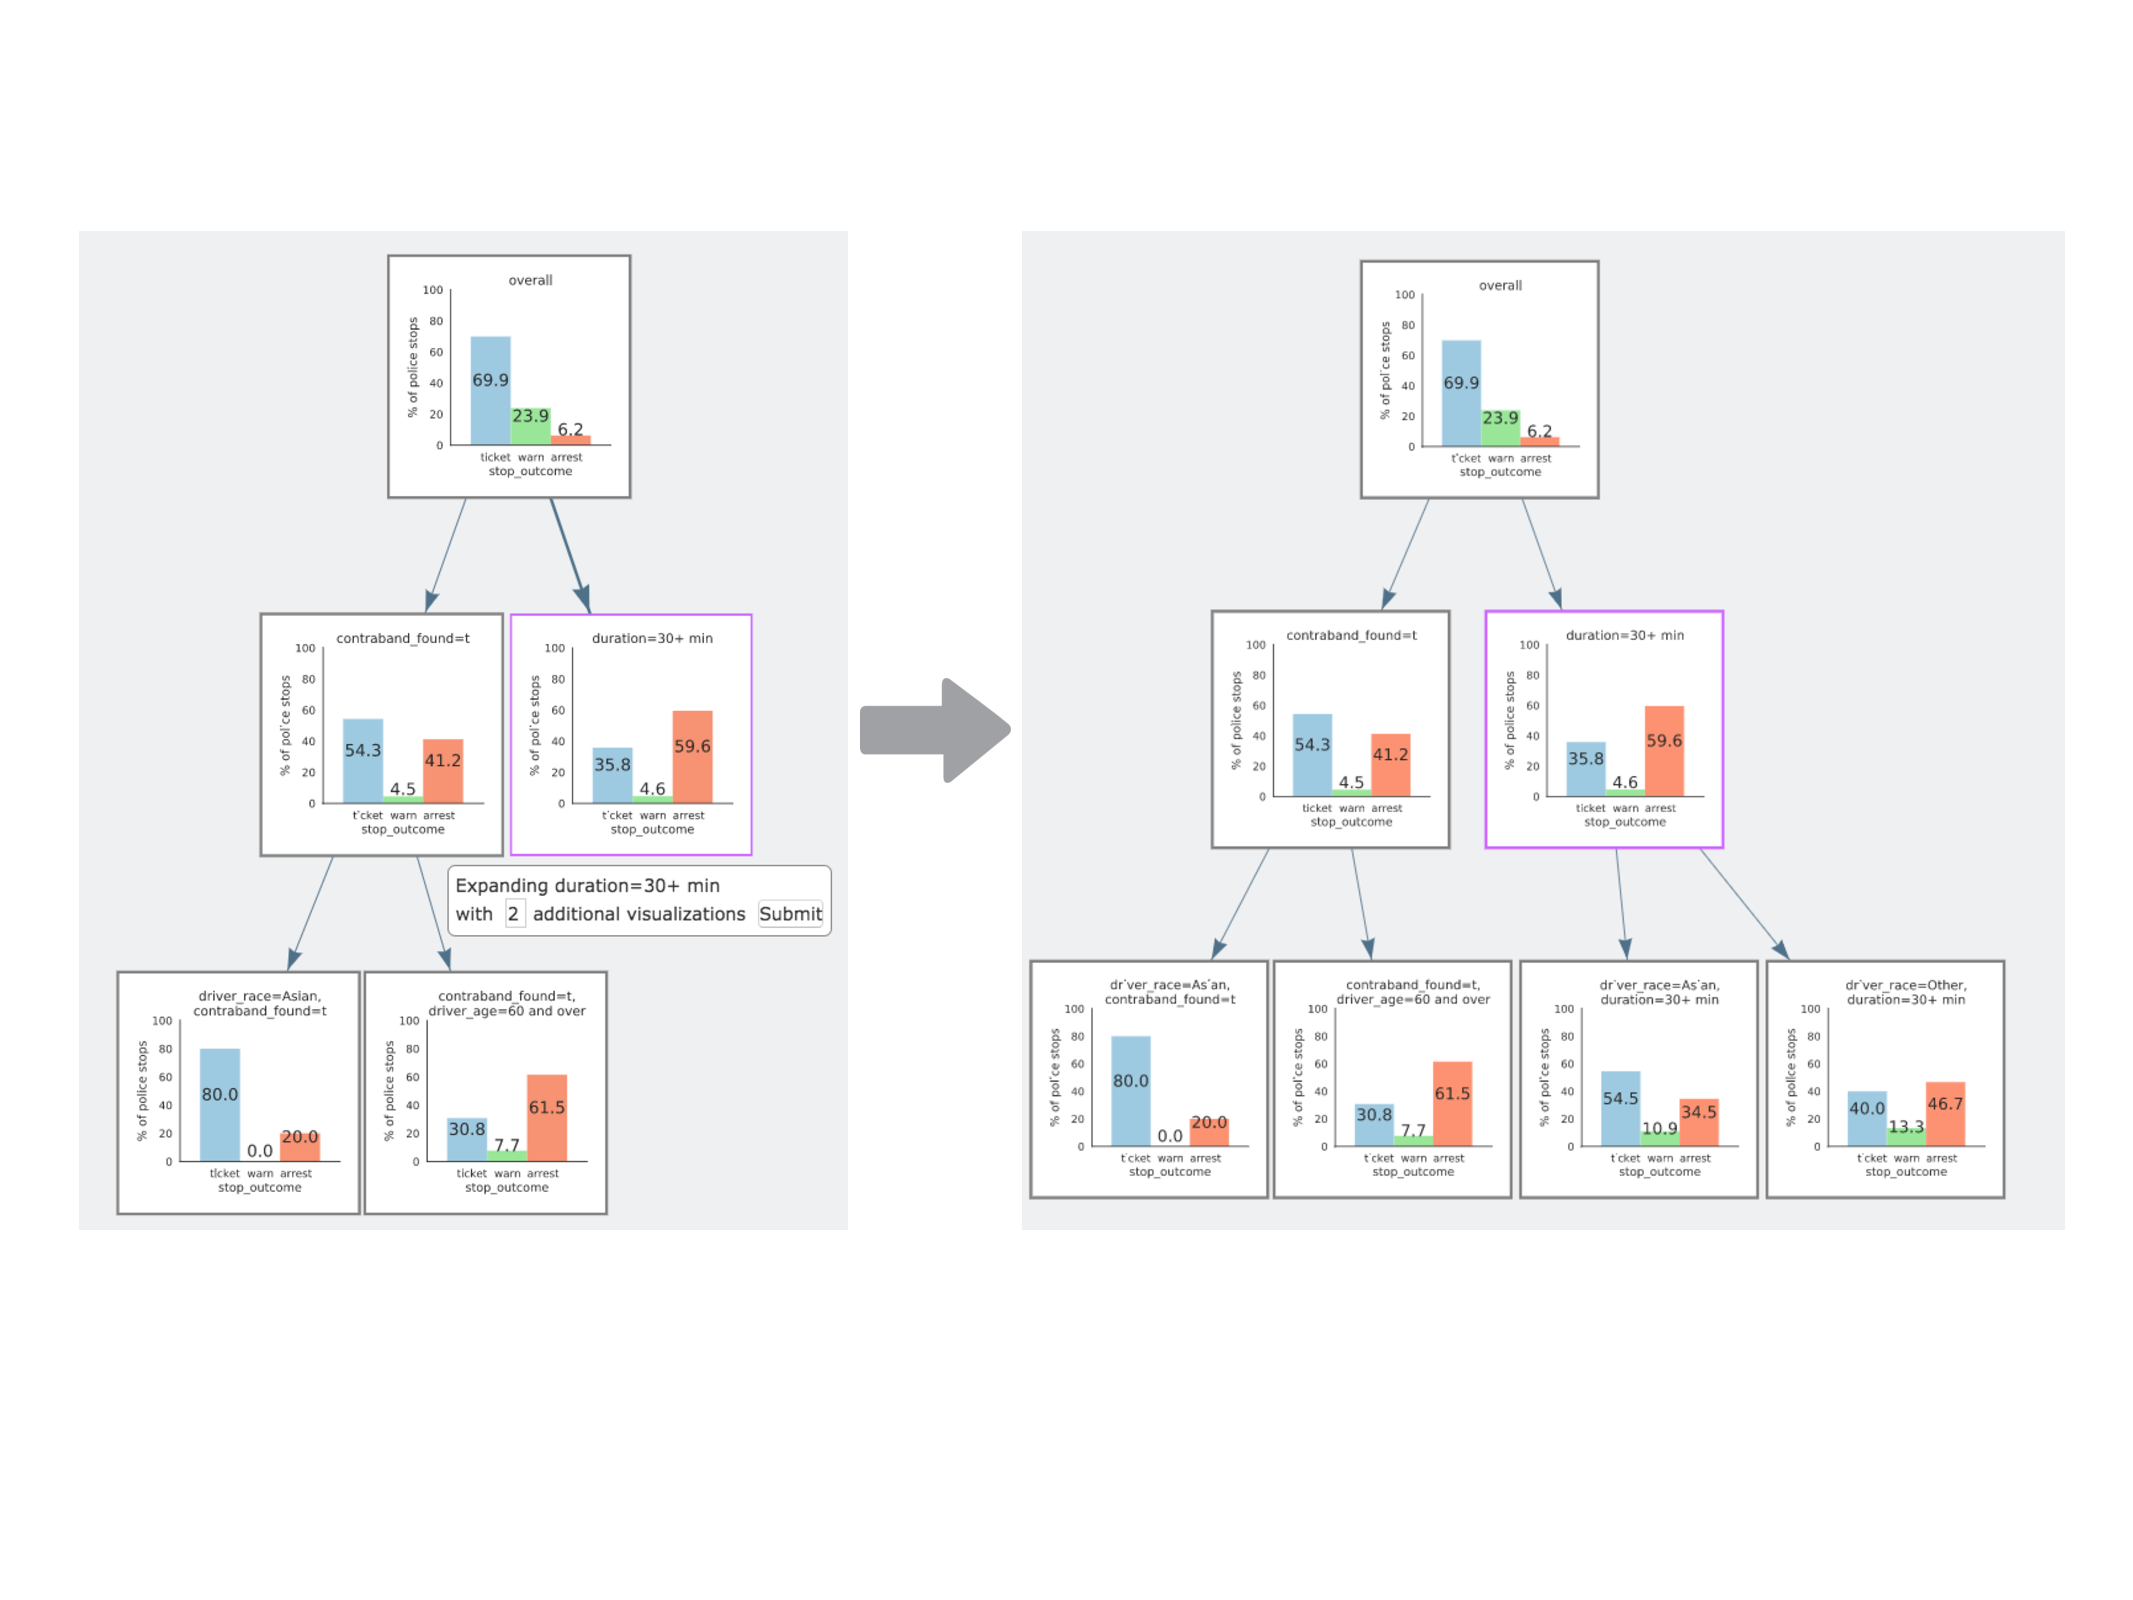
\includegraphics[width=\linewidth]{figures/expansion_example.pdf}
% \caption{Left: Original k=5 dashboard with the duration=30+min visualization clicked. A pop-up is displayed to submit the request for additional summary visualizations to be generated. Right: Resulting dashboard after requesting for 2 more visualizations based on the visualization of interest.}
% \label{fig:altroot_expansion}
% \end{figure}
\techreport{
  \subsection{Assistive tools for visualizing large lattices\label{sec:navigation}}
  Due to the amount of space occupied by the hierarchical layout when the number of visualizations gets large, we have developed tools to help users navigate through different parts of the dashboard interactively.
  \stitle{Navigation Minimap:}  When the user zooms in on the dashboard, an overview mini-map is shown on the upper left-hand side of the canvas to help users identify which region of the dashboard they are currently exploring, as shown in Figure \ref{fig:hover_minimap}.
  \stitle{Collapsed visualizations:}
  One observation that we found across several datasets was that many visualizations had identical distributions, which resulted in lots of wasted space. Apart from their attribute name, these visualizations are not very informative for the users, therefore, we offer an option to collapse these visualization, as demonstrated in Figure \ref{fig:collapse_demo}. A visualization can be collapsed if it has more than one redundant sibling and does not have any children, so that there are no hidden stories stemming from lower-level dependencies. As shown in Figure \ref{fig:hover_minimap}, collapsed nodes can be easily identified by an orange border and the details of which visualizations are in the collapsed node are displayed when the user hovers over the visualization.
  %\afterpage{%to enable footnote in caption
  \begin{figure}[ht!]
  \centering
  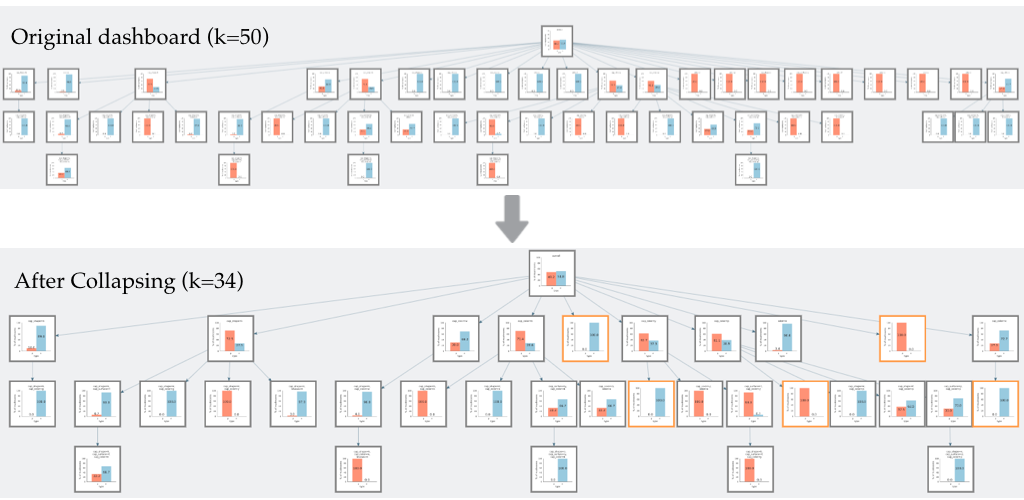
\includegraphics[width=\linewidth]{figures/collapsed_example.png}
  \caption{An example of the k=50 dashboard for the mushroom dataset~\cite{mushroom}, which contains type=\{posionous, edible\} on the x-axis. The collapsed dashboard (bottom) removed 16 redundant visualizations from the original dashboard (top).}
  \label{fig:collapse_demo}
  \end{figure}
  %}
  \begin{figure}[ht!]
  \centering
  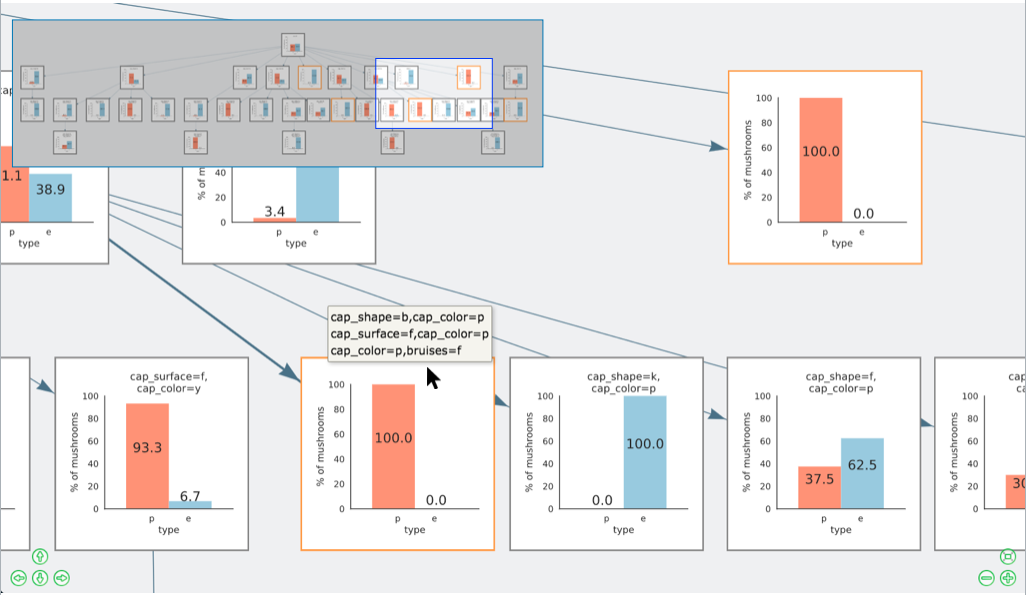
\includegraphics[width=\linewidth]{figures/minimap_zoom.png}
  \caption{Zoomed-in version of Figure \ref{fig:collapse_demo} showing the labels of a collapsed visualization when user hovers over the visualization. The navigation minimap is shown in the top-left to help users navigate through the large dashboard.}
  \label{fig:hover_minimap}
  \end{figure}
}
